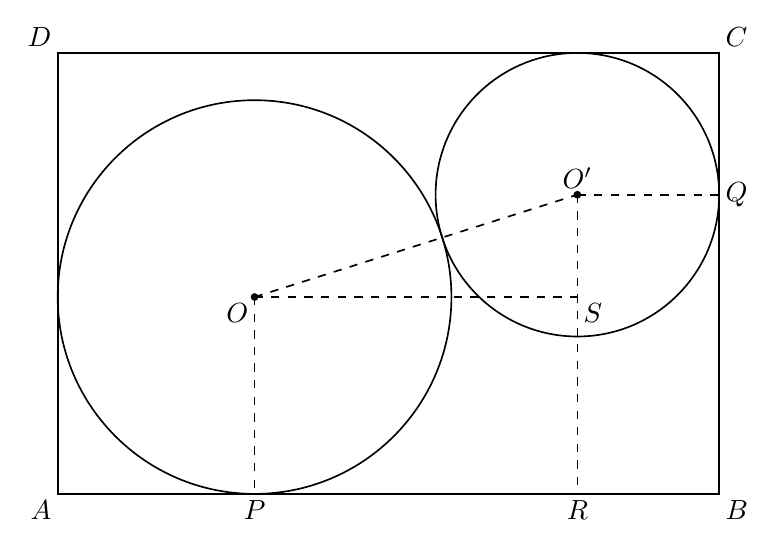
\begin{tikzpicture}[x=1cm,y=1cm,line width=.6pt,font=\normalsize]
\coordinate (A) at (0,0);
\coordinate (B) at (8.4,0);
\coordinate (C) at (8.4,5.6);
\coordinate (D) at (0,5.6);
\coordinate (O) at (2.5,2.5);
\coordinate (Oprime) at (6.5995,3.7995);
\coordinate (P) at (2.5,0);
\coordinate (R) at (6.5995,0);
\coordinate (S) at (6.5995,2.5);
\coordinate (Q) at (8.4,3.7995);
\draw (A)--(B)--(C)--(D)--cycle;
\draw (O) circle[radius=2.5cm];
\draw (Oprime) circle[radius=1.8005cm];
\draw[dashed] (O)--(Oprime);
\draw[dashed] (O)--(P);
\draw[dashed] (O)--(S);
\draw[dashed] (Oprime)--(R);
\draw[dashed] (Oprime)--(Q);
\node[below left=2pt,inner sep=0pt] at (A) {$A$};
\node[below right=2pt,inner sep=0pt] at (B) {$B$};
\node[above right=2pt,inner sep=0pt] at (C) {$C$};
\node[above left=2pt,inner sep=0pt] at (D) {$D$};
\node[below left=2pt,inner sep=0pt] at (O) {$O$};
\node[above=2pt,inner sep=0pt] at (Oprime) {$O'$};
\node[below=2pt,inner sep=0pt] at (P) {$P$};
\node[below=2pt,inner sep=0pt] at (R) {$R$};
\node[below right=2pt,inner sep=0pt] at (S) {$S$};
\node[right=2pt,inner sep=0pt] at (Q) {$Q$};

% Explicit named circle-center points, painted after all region fills.
\fill (O) circle[radius=1.4pt];
\fill (Oprime) circle[radius=1.4pt];
\end{tikzpicture}
